\documentclass{article}
\usepackage[utf8]{inputenc}
\usepackage[english]{babel}
\usepackage{amsmath,amsfonts,amssymb,amsthm}
\usepackage{mathtools}
\usepackage{fancyhdr}
\usepackage{commath}
\usepackage[sc,osf]{mathpazo}
\usepackage{graphicx}
\usepackage{rotating}
\usepackage{float}
\usepackage{subcaption}
\restylefloat{table}
\usepackage{multicol}
\usepackage[dvipsnames]{xcolor}
\usepackage[colorinlistoftodos]{todonotes}
\usepackage{vmargin}  % Administrar márgenes
\setpapersize{A4} % Definir tamaño del papel
\setmargins{2.5cm} % Margen izquierdo
{1cm} % Margen superior
{16.5cm} % Área de impresión horizontal
{23.42cm} % Area de impresión vertical
{15mm} % Encabezado
{5mm} % Espacio entre el encabezado y el texto
{10pt} % Pie de página
{3mm} % Espacio entre el pie de página y el texto

\pagestyle{fancy}
\fancyhf{}
\rhead{

\includegraphics[width=4cm,height=1cm]{cropped-iitpal-at-prutor-logo.png}
}
\lhead{Circles | Class XI}
\rfoot{}
\begin{document}
\section{Equation of Tangent}
To find tangent equation to the circle from a point $P(x_1,y_1)$ on it, use general form of circle. Since point $P$ is on circle,
\begin{equation*}
    x_1^2+y_1^2+2gx_1+2fy_1+c=0
\end{equation*}
\begin{figure}[H]
    \centering
    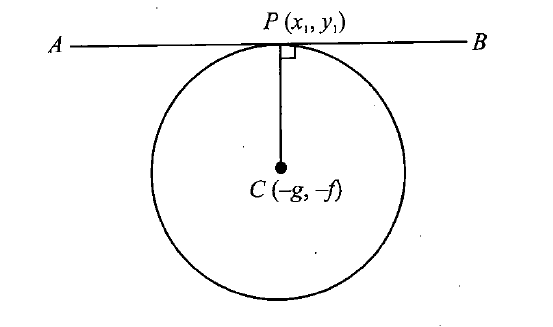
\includegraphics[scale=0.5]{tangent_on_circle.png}
    \caption{Tangent on Circle}
\end{figure}
Slope of line $CP$ can be given as,
\begin{equation*}
    \textbf{slope of CP} = \frac{y_1+f}{x_1+g}
\end{equation*}
As tangent $AB$ is perpendicular to $CP$,
\begin{equation*}
    \textbf{slope of tangent AB} = -\frac{x_1+g}{y_1+f}
\end{equation*}
Now we have slope of line $AB$ and it passes through point $P$, equation of tangent is,
\begin{equation*}
    y-y_1=-\frac{x_1+g}{y_1+f}(x-x_1)
\end{equation*}
\section{Length of Tangent from a given point}
Consider general form of circle $x^2+y^2+2gx+2fy+c=0$ with center $(-g,-f)$ and radius $\sqrt{g^2+f^2-c}$. Point is $P(x_1,y_1)$. Look at the diagram,
\begin{figure}[H]
    \centering
    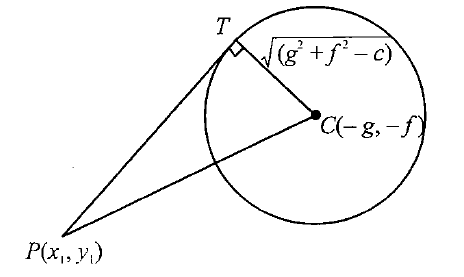
\includegraphics[scale=0.5]{length_of_tangent.png}
    \caption{Length of tangent}
\end{figure}
Length of $PC$,
\begin{equation*}
    PT=\sqrt{(PC)^2-(CP)^2}
\end{equation*}
Put value of $PC$ and $CP$, we get after solving
\begin{equation*}
    PT=\sqrt{x_1^2+y_1^2+2gx_1+2fy_1+c}
\end{equation*}
Put point value in general form of circle, and take its sq. root to get length of tangent from a point. 
\section{Equation of Normal}
Note that any normal on circle is a straight line which is perpendicular to the tangent that passes through center of the circle and point of contact on circle. Visualization of the same,
\begin{figure}[H]
    \centering
    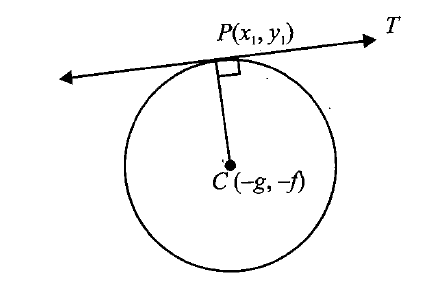
\includegraphics[scale=0.5]{normal_of_circle.png}
    \caption{Normal on Circle}
\end{figure}
Slope of $CP$,
\begin{equation*}
    \textbf{slope of CP} = \frac{y_1+f}{x_1+g}
\end{equation*}
Now we have slope of line $CP$ and it passes through point $P$, equation of normal is,
\begin{equation*}
    y-y_1=-\frac{y_1+f}{x_1+g}(x-x_1)
\end{equation*}
\end{document}